\documentclass{ximera}

 

\usepackage{epsfig}

\graphicspath{
  {./}
  {figures/}
}

\usepackage{morewrites}
\makeatletter
\newcommand\subfile[1]{%
\renewcommand{\input}[1]{}%
\begingroup\skip@preamble\otherinput{#1}\endgroup\par\vspace{\topsep}
\let\input\otherinput}
\makeatother

\newcommand{\includeexercises}{\directlua{dofile("/home/jim/linearAlgebra/laode/exercises.lua")}}

%\newcounter{ccounter}
%\setcounter{ccounter}{1}
%\newcommand{\Chapter}[1]{\setcounter{chapter}{\arabic{ccounter}}\chapter{#1}\addtocounter{ccounter}{1}}

%\newcommand{\section}[1]{\section{#1}\setcounter{thm}{0}\setcounter{equation}{0}}

%\renewcommand{\theequation}{\arabic{chapter}.\arabic{section}.\arabic{equation}}
%\renewcommand{\thefigure}{\arabic{chapter}.\arabic{figure}}
%\renewcommand{\thetable}{\arabic{chapter}.\arabic{table}}

%\newcommand{\Sec}[2]{\section{#1}\markright{\arabic{ccounter}.\arabic{section}.#2}\setcounter{equation}{0}\setcounter{thm}{0}\setcounter{figure}{0}}

\newcommand{\Sec}[2]{\section{#1}}

\setcounter{secnumdepth}{2}
%\setcounter{secnumdepth}{1} 

%\newcounter{THM}
%\renewcommand{\theTHM}{\arabic{chapter}.\arabic{section}}

\newcommand{\trademark}{{R\!\!\!\!\!\bigcirc}}
%\newtheorem{exercise}{}

\newcommand{\dfield}{{\sf dfield9}}
\newcommand{\pplane}{{\sf pplane9}}

\newcommand{\EXER}{\section*{Exercises}}%\vspace*{0.2in}\hrule\small\setcounter{exercise}{0}}
\newcommand{\CEXER}{}%\vspace{0.08in}\begin{center}Computer Exercises\end{center}}
\newcommand{\TEXER}{} %\vspace{0.08in}\begin{center}Hand Exercises\end{center}}
\newcommand{\AEXER}{} %\vspace{0.08in}\begin{center}Hand Exercises\end{center}}

% BADBAD: \newcommand{\Bbb}{\bf}

\newcommand{\R}{\mbox{$\Bbb{R}$}}
\newcommand{\C}{\mbox{$\Bbb{C}$}}
\newcommand{\Z}{\mbox{$\Bbb{Z}$}}
\newcommand{\N}{\mbox{$\Bbb{N}$}}
\newcommand{\D}{\mbox{{\bf D}}}
\usepackage{amssymb}
%\newcommand{\qed}{\hfill\mbox{\raggedright$\square$} \vspace{1ex}}
%\newcommand{\proof}{\noindent {\bf Proof:} \hspace{0.1in}}

\newcommand{\setmin}{\;\mbox{--}\;}
\newcommand{\Matlab}{{M\small{AT\-LAB}} }
\newcommand{\Matlabp}{{M\small{AT\-LAB}}}
\newcommand{\computer}{\Matlab Instructions}
\newcommand{\half}{\mbox{$\frac{1}{2}$}}
\newcommand{\compose}{\raisebox{.15ex}{\mbox{{\scriptsize$\circ$}}}}
\newcommand{\AND}{\quad\mbox{and}\quad}
\newcommand{\vect}[2]{\left(\begin{array}{c} #1_1 \\ \vdots \\
 #1_{#2}\end{array}\right)}
\newcommand{\mattwo}[4]{\left(\begin{array}{rr} #1 & #2\\ #3
&#4\end{array}\right)}
\newcommand{\mattwoc}[4]{\left(\begin{array}{cc} #1 & #2\\ #3
&#4\end{array}\right)}
\newcommand{\vectwo}[2]{\left(\begin{array}{r} #1 \\ #2\end{array}\right)}
\newcommand{\vectwoc}[2]{\left(\begin{array}{c} #1 \\ #2\end{array}\right)}

\newcommand{\ignore}[1]{}


\newcommand{\inv}{^{-1}}
\newcommand{\CC}{{\cal C}}
\newcommand{\CCone}{\CC^1}
\newcommand{\Span}{{\rm span}}
\newcommand{\rank}{{\rm rank}}
\newcommand{\trace}{{\rm tr}}
\newcommand{\RE}{{\rm Re}}
\newcommand{\IM}{{\rm Im}}
\newcommand{\nulls}{{\rm null\;space}}

\newcommand{\dps}{\displaystyle}
\newcommand{\arraystart}{\renewcommand{\arraystretch}{1.8}}
\newcommand{\arrayfinish}{\renewcommand{\arraystretch}{1.2}}
\newcommand{\Start}[1]{\vspace{0.08in}\noindent {\bf Section~\ref{#1}}}
\newcommand{\exer}[1]{\noindent {\bf \ref{#1}}}
\newcommand{\ans}{}
\newcommand{\matthree}[9]{\left(\begin{array}{rrr} #1 & #2 & #3 \\ #4 & #5 & #6
\\ #7 & #8 & #9\end{array}\right)}
\newcommand{\cvectwo}[2]{\left(\begin{array}{c} #1 \\ #2\end{array}\right)}
\newcommand{\cmatthree}[9]{\left(\begin{array}{ccc} #1 & #2 & #3 \\ #4 & #5 &
#6 \\ #7 & #8 & #9\end{array}\right)}
\newcommand{\vecthree}[3]{\left(\begin{array}{r} #1 \\ #2 \\
#3\end{array}\right)}
\newcommand{\cvecthree}[3]{\left(\begin{array}{c} #1 \\ #2 \\
#3\end{array}\right)}
\newcommand{\cmattwo}[4]{\left(\begin{array}{cc} #1 & #2\\ #3
&#4\end{array}\right)}

\newcommand{\Matrix}[1]{\ensuremath{\left(\begin{array}{rrrrrrrrrrrrrrrrrr} #1 \end{array}\right)}}

\newcommand{\Matrixc}[1]{\ensuremath{\left(\begin{array}{cccccccccccc} #1 \end{array}\right)}}



\renewcommand{\labelenumi}{\theenumi)}
\newenvironment{enumeratea}%
{\begingroup
 \renewcommand{\theenumi}{\alph{enumi}}
 \renewcommand{\labelenumi}{(\theenumi)}
 \begin{enumerate}}
 {\end{enumerate}\endgroup}



\newcounter{help}
\renewcommand{\thehelp}{\thesection.\arabic{equation}}

%\newenvironment{equation*}%
%{\renewcommand\endequation{\eqno (\theequation)* $$}%
%   \begin{equation}}%
%   {\end{equation}\renewcommand\endequation{\eqno \@eqnnum
%$$\global\@ignoretrue}}

%\input{psfig.tex}

\author{Martin Golubitsky and Michael Dellnitz}

%\newenvironment{matlabEquation}%
%{\renewcommand\endequation{\eqno (\theequation*) $$}%
%   \begin{equation}}%
%   {\end{equation}\renewcommand\endequation{\eqno \@eqnnum
% $$\global\@ignoretrue}}

\newcommand{\soln}{\textbf{Solution:} }
\newcommand{\exercap}[1]{\centerline{Figure~\ref{#1}}}
\newcommand{\exercaptwo}[1]{\centerline{Figure~\ref{#1}a\hspace{2.1in}
Figure~\ref{#1}b}}
\newcommand{\exercapthree}[1]{\centerline{Figure~\ref{#1}a\hspace{1.2in}
Figure~\ref{#1}b\hspace{1.2in}Figure~\ref{#1}c}}
\newcommand{\para}{\hspace{0.4in}}

\renewenvironment{solution}{\suppress}{\endsuppress}

\ifxake
\newenvironment{matlabEquation}{\begin{equation}}{\end{equation}}
\else
\newenvironment{matlabEquation}%
{\let\oldtheequation\theequation\renewcommand{\theequation}{\oldtheequation*}\begin{equation}}%
  {\end{equation}\let\theequation\oldtheequation}
\fi

\makeatother


\title{Sinks, Saddles, and Sources}

\begin{document}
\begin{abstract}
\end{abstract}
\maketitle

 \label{S:6.7}

The qualitative theory of autonomous differential equations begins with
the observation that many important properties of solutions to constant
coefficient systems of differential equations
\begin{equation} \label{e:C2}
\frac{dX}{dt}=CX
\end{equation}
are unchanged by similarity.

Begin by noting that the origin is always an equilibrium for \eqref{e:C2}
and suppose that $C$ is a $2\times 2$ matrix.  The origin for \eqref{e:C2}
is called a {\em sink\/}\index{sink} if the eigenvalues of $C$ both have
negative real
part and a {\em source\/}\index{source} if the eigenvalues both have
positive real part.
When $C$ has one eigenvalue of each sign, the origin is called a
{\em saddle}\index{saddle}.

Now suppose that $B$ is a $2\times 2$ matrix that is similar to $C$.
Lemma~\ref{L:simdettr} of Chapter~\ref{Chap:Planar} states that $B$ and
$C$ have the same eigenvalues.  It follows that if the origin is a saddle
for \eqref{e:C2}, then it is a saddle for $\dot{X}=BX$.  Similar statements
hold for sinks and sources.

\subsection*{Asymptotic Stability}

We now discuss asymptotic stability of the origin in linear systems.
Recall from our discussion in Section~\ref{sec:UncoupledLS} 
that the origin is {\em asymptotically stable\/} \index{stability!asymptotic}
if every trajectory $X(t)$ beginning at an initial condition near the
origin stays near $0$ for all positive $t$, and
\[
\lim_{t\to\infty}X(t) = 0.
\]
Recall also from Lemma~\ref{L:simsoln} that
if $B=P\inv CP$, then $P\inv X(t)$ is a solution to $\dot{X}=BX$ whenever
$X(t)$ is a solution to \eqref{e:C2}.  Since $P\inv$ is a matrix of constants
that do not depend on $t$, it follows that
\[
\lim_{t\to\infty}X(t) = 0 \Longleftrightarrow \lim_{t\to\infty}P\inv X(t) = 0.
\]
So the origin is asymptotically stable for $\dot{X}=BX$ if and only if it is
asymptotically stable for \eqref{e:C2}.  With this observation in hand, we
prove that sinks are stable.

\begin{theorem}  \label{C:asympstlin}
If the eigenvalues of a $2\times 2$ matrix $C$ has negative real part, then 
the origin is an asymptotically stable equilibrium\index{equilibrium} for \eqref{e:C2}.
If one of the
eigenvalues of $C$ has positive real part, then the origin is unstable.
\end{theorem}

\begin{proof}  This proof is based on the closed form of solutions given in
Section~\ref{S:6.5}.   The remark preceding this theorem states that we
need only prove this theorem for differential equations up to similarity.

\noindent (a) \quad If the eigenvalues $\lambda_1$ and $\lambda_2$ are real
and there are two independent eigenvectors, then Chapter~\ref{Chap:Planar},
Theorem~\ref{T:putinform} states that the matrix $C$ is similar to the
diagonal matrix
\[
B = \mattwoc{\lambda_1}{0}{0}{\lambda_2}.
\]
The general solution to the differential equation $\dot{X}=BX$ is
\[
x_1(t) = \alpha_1e^{\lambda_1 t} \AND x_2(t) = \alpha_2e^{\lambda_2 t}.
\]
Since
\[
\lim_{t\to\infty}e^{\lambda_1 t} = 0  = \lim_{t\to\infty}e^{\lambda_2 t},
\]
when $\lambda_1$ and $\lambda_2$ are negative, it follows that
\[
\lim_{t\to\infty} X(t) = 0
\]
for all solutions $X(t)$, and the origin is asymptotically stable.  Note that
if one of the eigenvalues, say $\lambda_1$, is positive then $x_1(t)$ will
undergo exponential growth and the origin is unstable.

\noindent (b) \quad If the eigenvalues of $C$ are the complex conjugates
$\sigma\pm i\tau$ where $\tau\neq 0$, then Chapter~\ref{Chap:Planar},
Theorem~\ref{T:putinform} states that after a similarity transformation
\eqref{e:C2} has the form
\[
\dot{X} = \mattwo{\sigma}{-\tau}{\tau}{\sigma}X,
\]
and solutions for this equation have the form \eqref{e:exp0ev} of
Chapter~\ref{Chap:Planar}, that is,
\[
X(t) = e^{\sigma t}
\mattwo{\cos(\tau t)}{-\sin(\tau t)}{\sin(\tau t)}{\cos(\tau t)}X_0
= e^{\sigma t}R_{\tau t}X_0,
\]
where $R_{\tau t}$ is a rotation matrix\index{rotation!matrix}
(recall \eqref{e:rotmat} of
Chapter~\ref{chap:matrices}).  It follows that as time evolves
the vector $X_0$ is rotated about the origin and then expanded or contracted
by the factor $e^{\sigma t}$.  So when $\sigma<0$, $\lim_{t\to\infty} X(t)=0$
for all solutions $X(t)$.  Hence the origin is asymptotically stable.  Note
that when $\sigma>0$ solutions spiral away from the origin.

\noindent (c) \quad If the eigenvalues are both equal to $\lambda_1$
and if there is only one independent eigenvector, then
Chapter~\ref{Chap:Planar}, Theorem~\ref{T:putinform} states that after a
similarity transformation \eqref{e:C2} has the form
\[
\dot{X} = \mattwo{\lambda_1}{1}{0}{\lambda_1}X,
\]
whose solutions are
\[
X(t) = e^{t\lambda}\mattwoc{1}{t}{0}{1} X_0
\]
using Table~\ref{T:3sys}(c). Note that the functions
$e^{\lambda_1 t} \AND te^{\lambda_1 t}$ both have limits equal to zero as
$t\to\infty$.  In the second case, use l'H\^{o}spital's rule and the
assumption that $-\lambda_1>0$ to compute
\[
\lim_{t\to\infty} \frac{t}{e^{-\lambda_1 t}} =
  -\lim_{t\to\infty} \frac{1}{\lambda_1 e^{-\lambda_1 t}} = 0.
\]
Hence $\lim_{t\to\infty} X(t) =0$ for all solutions $X(t)$ and the origin
is asymptotically stable.  Note that initially $||X(t)||$ can grow since
$t$ is increasing.  But eventually exponential decay wins out and solutions
limit on the origin.   Note that solutions grow exponentially when
$\lambda_1>0$.  \end{proof}

It is instructive to note how the time series $x_1(t)$ damps down to the
origin in the three cases listed in Theorem~\ref{C:asympstlin}.
In Figure~\ref{F:oscil} we present the time series for the three
coefficient matrices:
\begin{align*}
C_1 &= \mattwo{-2}{0}{0}{-1}, \\
C_2 &= \mattwo{-1}{-55}{55}{-1}, \\
C_3 &= \mattwo{-2}{1}{0}{-2}.
\end{align*}
In this figure, we can see the exponential decay to zero associated with the
unequal real eigenvalues of $C_1$; the damped oscillation associated with the
complex eigenvalues of $C_2$; and the initial growth of the time series due
to the $te^{-2t}$ term followed by exponential decay to zero in the equal
eigenvalue $C_3$ example.

\begin{figure*}[htb]
           \centerline{%
           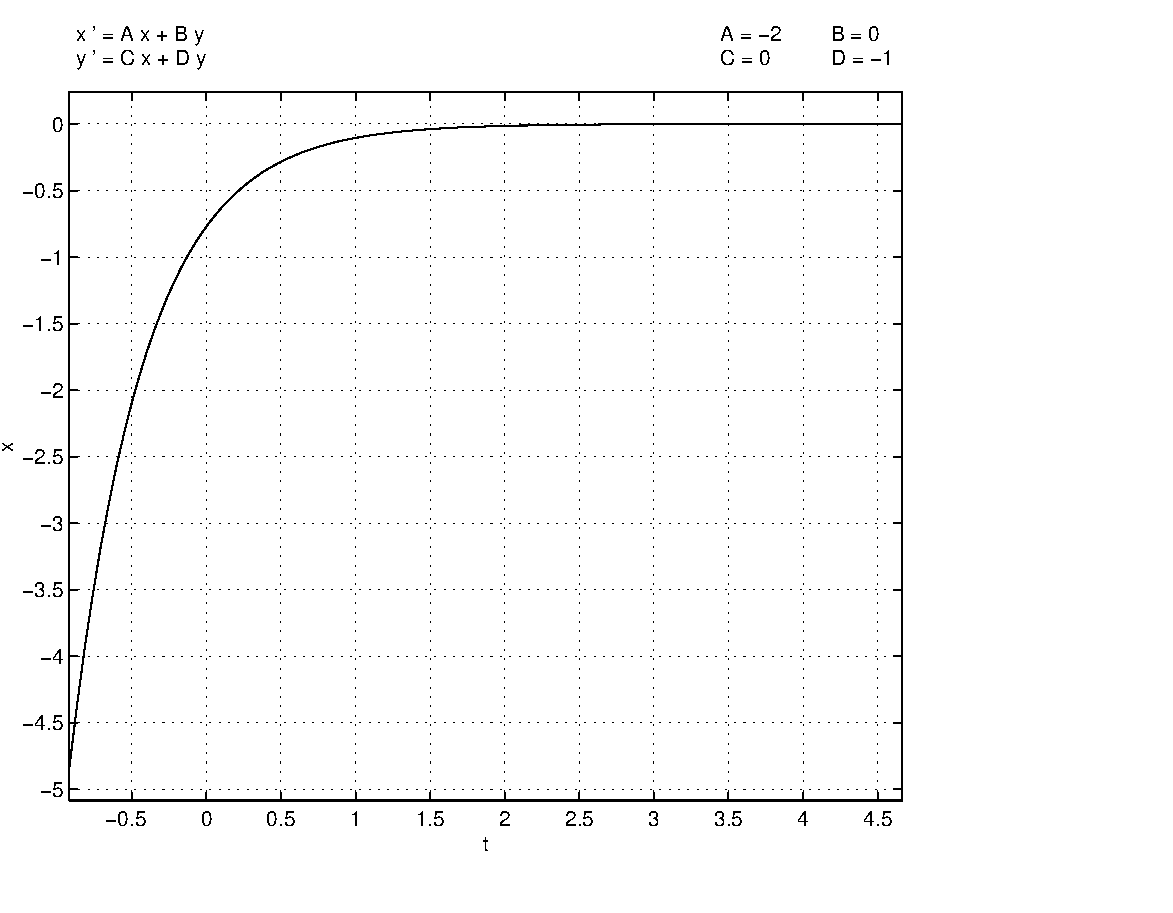
\psfig{file=../figures/expdamp.eps,width=2.2in}
	   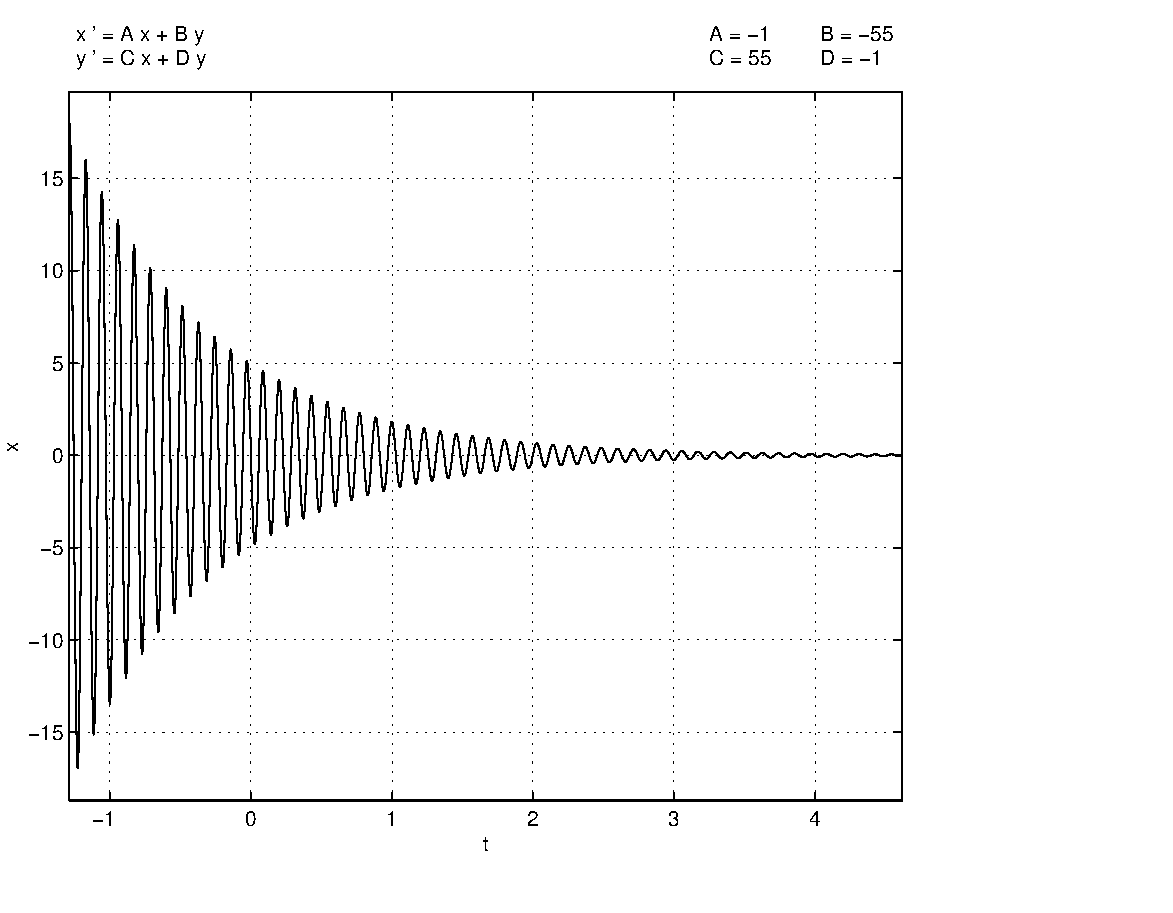
\psfig{file=../figures/oscil.eps,width=2.2in}
	   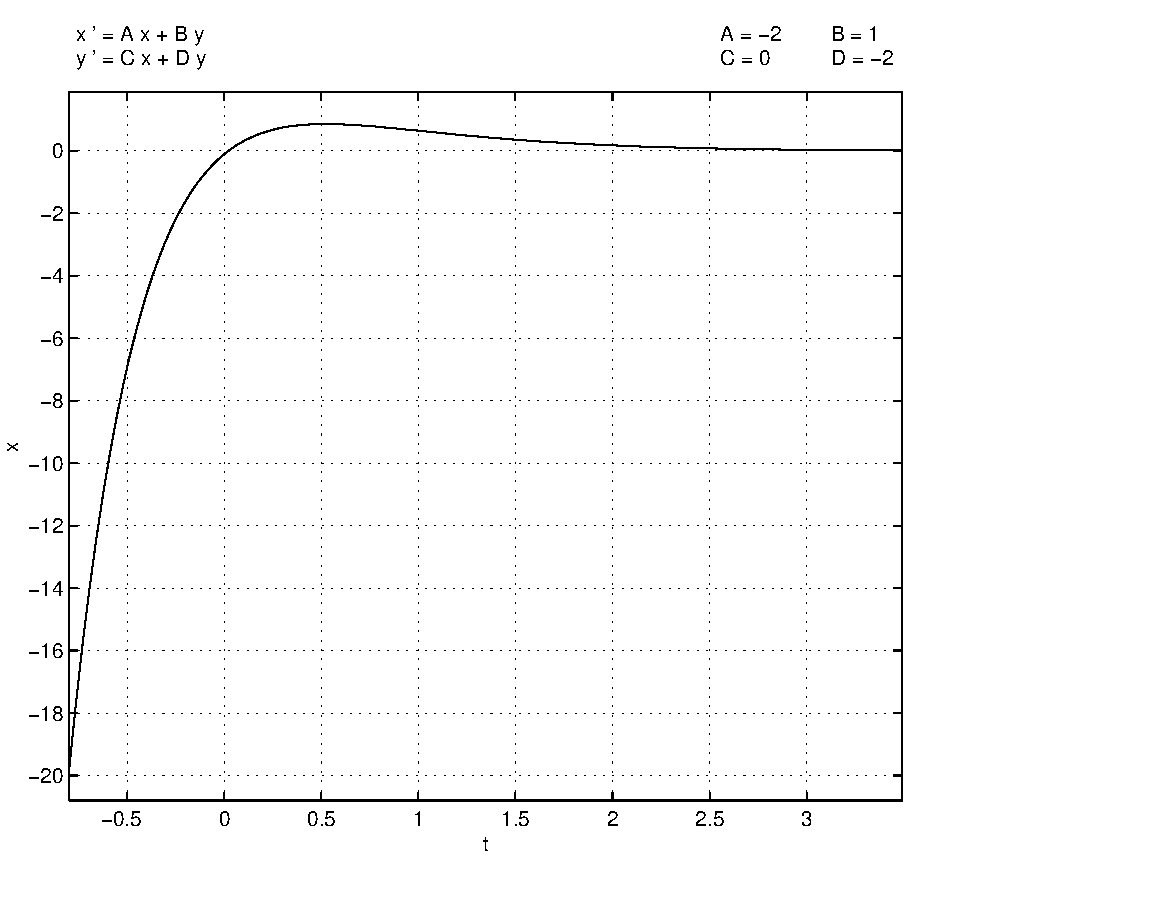
\psfig{file=../figures/grdecay.eps,width=2.2in}}
           \caption{Time series for different sinks.}
           \label{F:oscil}
\end{figure*}


\subsubsection*{Linear Stability}

Saddles, sinks, and sources are distinguished by the stability of the
origin.  In Theorem~\ref{C:asympstlin} we showed that the origin is
asymptotically stable if the eigenvalues have negative real part, that is,
if the origin is a sink.  There is another term that is commonly used and
is synonymous with sink.
\begin{definition} \label{D:linstablin}
The origin is a {\em linearly stable\/} equilibrium of \eqref{e:C2} if the
eigenvalues of $C$ have negative real part.
\end{definition}\index{stability!linear}
So Theorem~\ref{C:asympstlin} may be restated as: linear stability
implies asymptotic stability of the origin.

\subsubsection*{Sources Versus Sinks}

The explicit form of solutions to planar linear systems shows that solutions
with initial conditions near the origin grow exponentially in forward time
when the origin of \eqref{e:C2} is a source.  We can prove this point
geometrically, as follows.

The phase planes of sources and sinks are almost the same; they have the
same trajectories but the arrows are reversed.  To verify this point, note
that
\begin{equation}  \label{e:C3}
\dot{X}=-CX
\end{equation}
is a sink when \eqref{e:C2} is a source; observe that the trajectories of
solutions of \eqref{e:C2} are the same as those of \eqref{e:C3} --- just with
time running backwards.  For let $X(t)$ be a solution to \eqref{e:C2}; then
$X(-t)$ is a solution to \eqref{e:C3}.   See Figure~\ref{F:SS} for plots of
$\dot{X}=BX$ and $\dot{X}=-BX$ where
\begin{equation}  \label{E:SS}
B = \mattwo{-1}{-5}{5}{-1}.
\end{equation}

So when we draw schematic phase portraits\index{phase!portrait}
for sinks\index{phase!portrait!for a sink}, we automatically know
how to draw schematic phase portraits for
sources\index{phase!portrait!for a source}.  The trajectories are
the same --- but the arrows point in the opposite direction.

\begin{figure*}[htb]
           \centerline{%
	   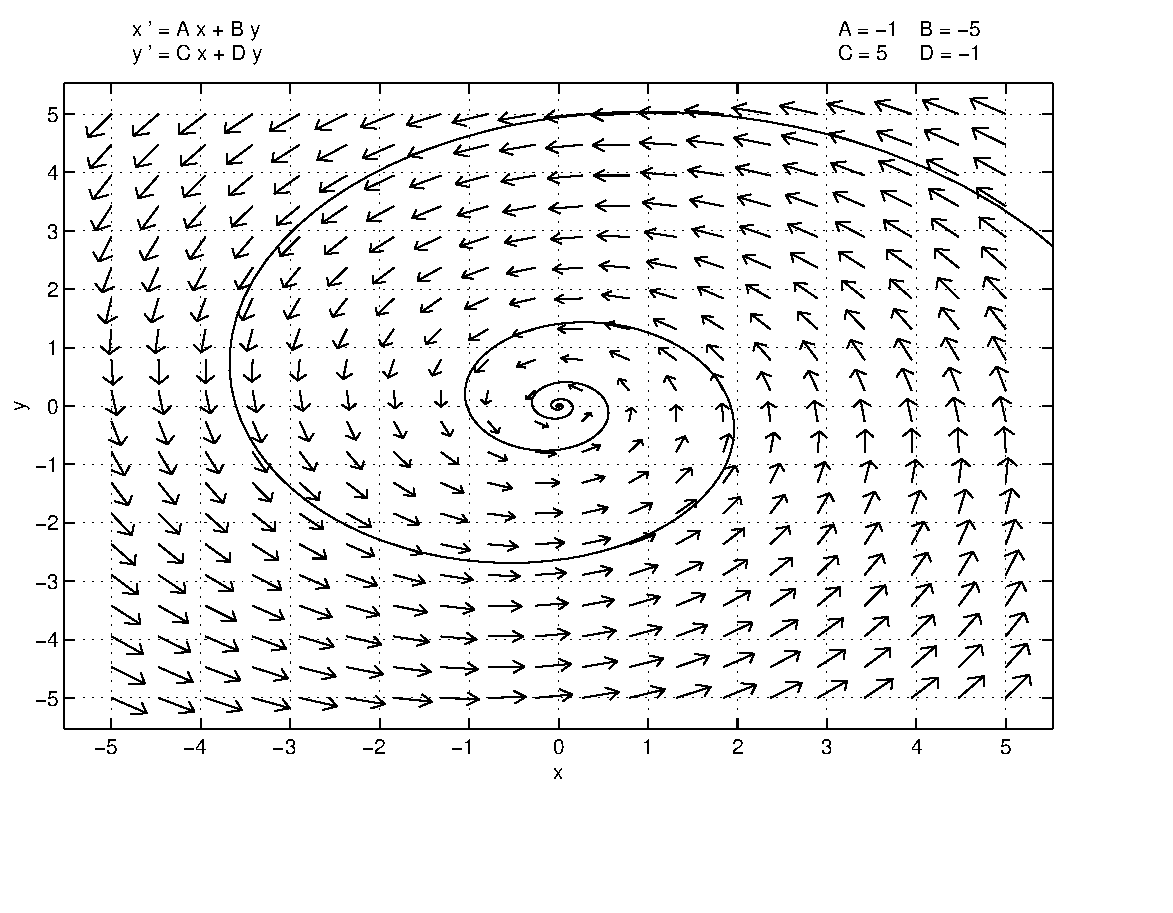
\psfig{file=../figures/asink.eps,width=3.2in}
           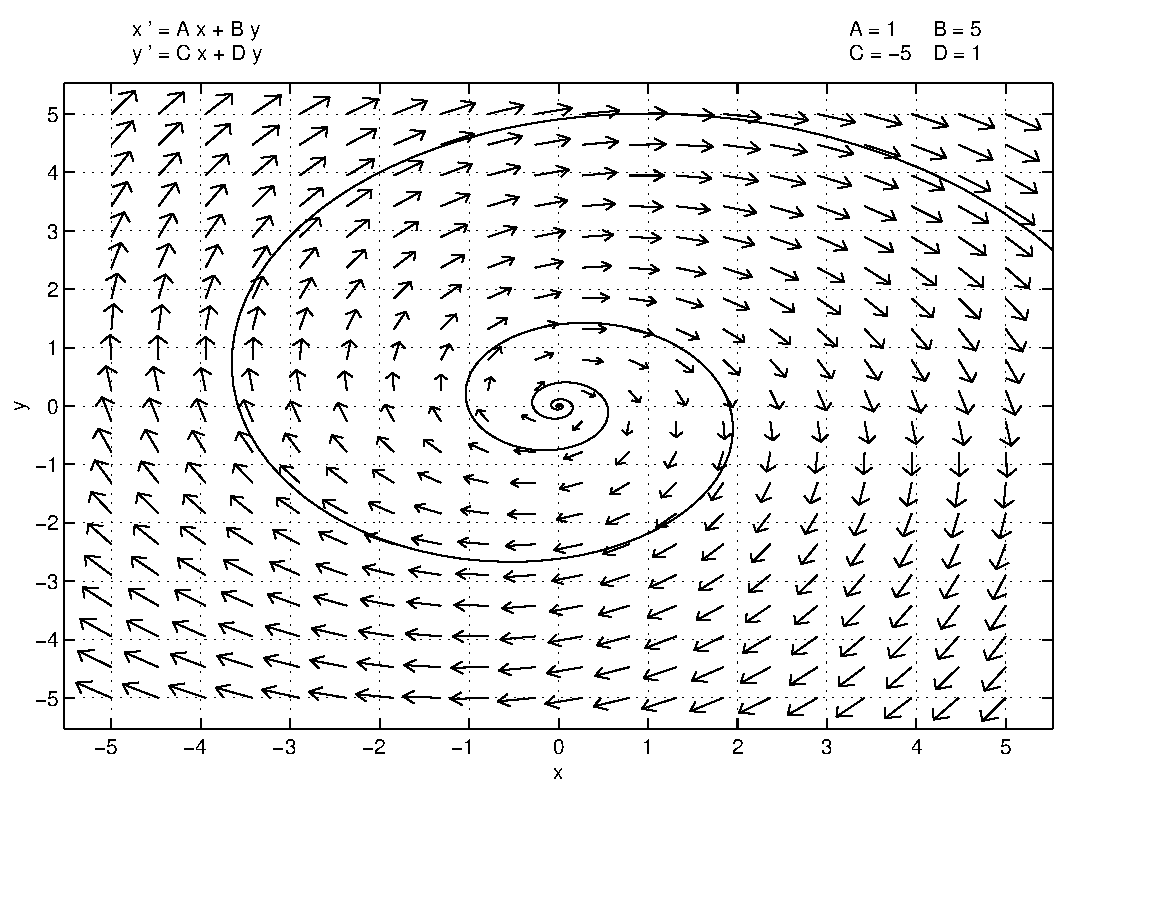
\psfig{file=../figures/asource.eps,width=3.2in}}
           \caption{(Left) Sink $\dot{X}=BX$ where $B$ is given in
\protect{\eqref{E:SS}}.  (Right) Source $\dot{X}=-BX$.}
           \label{F:SS}
\end{figure*}


\subsection*{Phase Portraits for Saddles}
\index{phase!portrait!for a saddle}

Next we discuss the phase portraits of linear saddles.  Using
{\sf pplane8}\index{\computer!pplane8}, draw the phase portrait
of the saddle
\begin{equation}  \label{e:saddlet}
\begin{array}{rcl}
\dot{x} & = & 2x+y\\
\dot{y} & = & -x-3y,
\end{array}
\end{equation}
as in Figure~\ref{F:linsaddle}.  The important feature of saddles
is that there are special trajectories (the eigendirections) that
limit on the origin in either forward or backward time.

\begin{figure*}[htb]
           \centerline{%
	   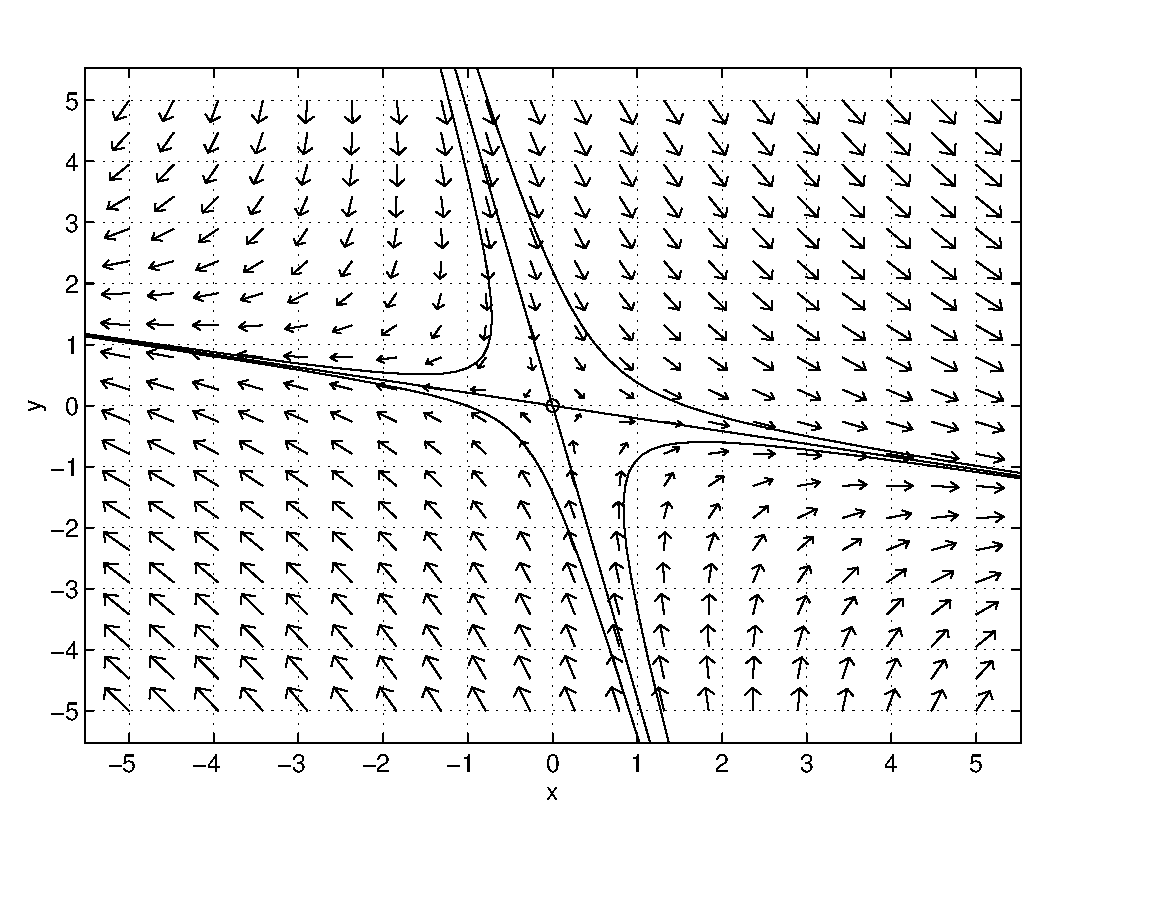
\psfig{file=../figures/linpnb.eps,width=3.5in}
           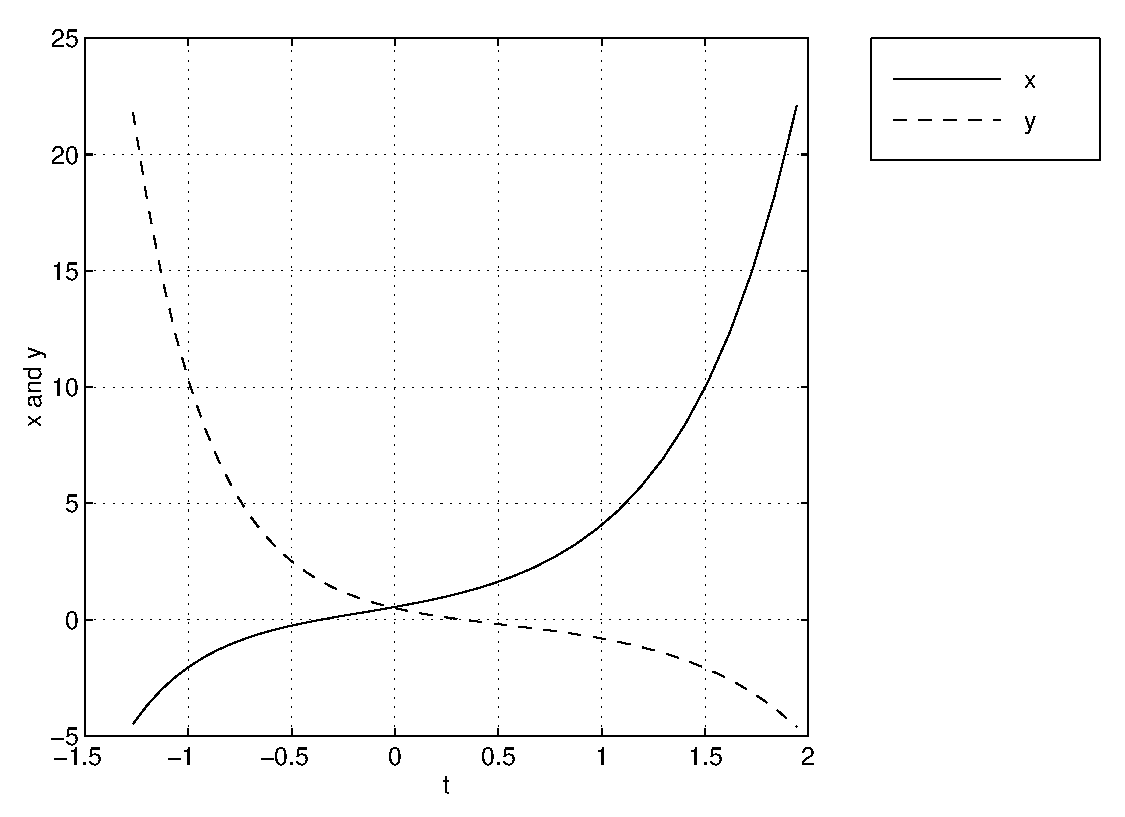
\psfig{file=../figures/linpnts.eps,width=3.5in}}
           \caption{(Left) Saddle phase portrait.
	(Right) First quadrant solution time series.}
           \label{F:linsaddle}
\end{figure*}

\begin{definition} \label{D:stablemfld}
The {\em stable manifold\/} or {\em stable orbit\/} of a saddle consists of
those trajectories that limit on the origin in forward time; the
{\em unstable manifold\/} or {\em unstable orbit\/} of a saddle consists of
those trajectories that limit on the origin in backward time.
\end{definition}
\index{stable!manifold} \index{unstable!manifold}
\index{stable!orbit} \index{unstable!orbit}

Let $\lambda_1<0$ and $\lambda_2>0$ be the eigenvalues of a saddle with
associated eigenvectors $v_1$ and $v_2$.  The stable orbits are given by the
solutions $X(t) = \pm e^{\lambda_1 t}v_1$ and the unstable orbits are given
by the solutions $X(t) = \pm e^{\lambda_2 t}v_2$.

\subsubsection*{Stable and Unstable Orbits using {\sf pplane8}}

The program {\sf pplane8} is programmed to draw the stable and unstable
orbits of a saddle on command. Although the principal use of this
feature is seen when analyzing nonlinear systems, it is useful to
introduce this feature here.  As an example, load the linear system
\eqref{e:saddlet} into {\sf pplane8} and click on {\sf Proceed}.  Now
pull down the {\sf PPLANE8 Options} menu and click on {\sf Find an
equilibrium}.  Click the cross hairs in the {\sf PPLANE8 Display}
window on a point near the origin; {\sf pplane8} responds by
opening a new window --- the {\sf PPLANE8 Equilibrium point data}
window --- and by putting a small yellow circle about the
origin.  The circle indicates that the numerical algorithm
programmed into {\sf pplane8} has detected an equilibrium near
the chosen point. A new window opens and displays the message
{\sf There is a saddle point at} $(0,0)$.  This window also displays the
coefficient matrix (called the {\em Jacobian} at the equilibrium) and its eigenvalues
and eigenvectors.  This process numerically verifies that the origin
is a saddle (a fact that could have been verified in a more
straightforward way).

Now pull down the {\sf PPLANE8 Options} menu again and click on
{\sf Plot stable and unstable orbits}.  Next click on the mouse
when the cross hairs are within the yellow circle and {\sf
pplane8} responds by drawing the stable and unstable orbits.
The result is shown in Figure~\ref{F:linsaddle}(left).
On this figure we have also plotted one trajectory
from each quadrant; thus obtaining the phase portrait of a saddle.
On the right of Figure~\ref{F:linsaddle} we have plotted a
time series of the first quadrant solution.  Note how the $x$
time series increases exponentially to $+\infty$ in forward time and 
the $y$ time series decreases in forward time while going exponentially 
towards $-\infty$.  The two time series together
give the trajectory $(x(t),y(t))$ that in forward time is asymptotic
to the line given by the unstable eigendirection.



\EXER

\TEXER


\noindent In Exercises~\ref{E:stabmata} -- \ref{E:stabmatc} determine
whether or not the equilibrium at the origin in the system of differential
equations $\dot{X}=CX$ is asymptotically stable.
\begin{exercise} \label{E:stabmata}
$C=\mattwo{1}{2}{4}{1}$.

\begin{solution}
\ans The origin is not asymptotically stable.

\soln Theorem~\ref{C:asympstlin} states that the origin is a stable
equilibrium only if all eigenvectors have negative real part.  The
characteristic polynomial of $C$ is $p_C(\lambda) = \lambda^2 - 2\lambda
- 5$.  Thus, the eigenvalues are $\lambda_1 = 1 + \sqrt{6}$ and
$\lambda_2 = 1 - \sqrt{6}$. Since $\lambda_1 > 0$, the origin
is not stable.

\end{solution}
\end{exercise}
\begin{exercise} \label{E:stabmatb}
$C=\mattwo{-1}{2}{-4}{-1}$.

\begin{solution}
\ans The origin is asymptotically stable.

\soln The characteristic polynomial of the matrix is $p_C(\lambda) =
\lambda^2 + 2\lambda + 7$.  Thus, the eigenvalues are $\lambda_1 =
-1 + 2\sqrt{2}i$ and $\lambda_2 = -1 - 2\sqrt{2}i$.  Both of these
have negative real part, so the origin is stable.

\end{solution}
\end{exercise}
\begin{exercise} \label{E:stabmatc}
$C=\mattwo{2}{1}{1}{-5}$.

\begin{solution}
\ans The origin is not asymptotically stable.

\soln The characteristic polynomial of the matrix is $p_C(\lambda) =
\lambda^2 - 3\lambda - 11$.  Thus, the eigenvalues are $\lambda_1 =
\frac{3}{2} + \sqrt{53}$ and $\lambda_2 = \frac{3}{2} - \sqrt{53}$.
Since $\lambda_1 > 0$, the origin is not stable.

\end{solution}
\end{exercise}

\noindent In Exercises~\ref{E:sisasoa} -- \ref{E:sisasof} determine
whether the equilibrium at the origin in the system of differential
equations $\dot{X}=CX$ is a sink, a saddle or a source.
\begin{exercise} \label{E:sisasoa}
$C=\mattwo{-2}{2}{0}{-1}$.

\begin{solution}
\ans The origin of the system $\dot{X} = CX$ is a sink.

\soln The characteristic polynomial of $C$ is
$p_C(\lambda) = \lambda^2 + 3\lambda + 2$.  So the eigenvalues are
$\lambda_1 = -1$ and $\lambda_2 = -2$.  Since both eigenvalues have
negative real part, the origin is a sink.

\end{solution}
\end{exercise}
\begin{exercise} \label{E:sisasob}
$C=\mattwo{3}{5}{0}{-2}$.

\begin{solution}
\ans The origin of the system $\dot{X} = CX$ is a saddle.

\soln The characteristic polynomial of $C$ is
$p_C(\lambda) = \lambda^2 - \lambda - 6$.  So the eigenvalues are
$\lambda_1 = 3$ and $\lambda_2 = -2$.  Since one eigenvalue is negative
and one is positive, the origin is a saddle.

\end{solution}
\end{exercise}
\begin{exercise} \label{E:sisasoc}
$C=\mattwo{4}{2}{-1}{2}$.

\begin{solution}
\ans The origin of the system $\dot{X} = CX$ is a source.

\soln The characteristic polynomial of $C$ is
$p_C(\lambda) = \lambda^2 - 6\lambda + 10$.  So the eigenvalues are
$\lambda = 3 \pm i$.  Since both eigenvalues have positive real part,
the origin is a source.

\end{solution}
\end{exercise}
\begin{exercise} \label{E:sisasod}
$C=\mattwo{8}{0}{-5}{3}$.

\begin{solution}
\ans The origin of the system $\dot{X} = CX$ is a source.

\soln The characteristic polynomial of $C$ is
$p_C(\lambda) = \lambda^2 - 11\lambda + 24$.  So the eigenvalues are
$\lambda_1 = 8$ and $\lambda_2 = 3$.  Since both eigenvalues have
positive real part, the origin is a source.

\end{solution}
\end{exercise}
\begin{exercise} \label{E:sisasoe}
$C=\mattwo{9}{-11}{-11}{9}$.

\begin{solution}
\ans The origin of the system $\dot{X} = CX$ is a saddle.

\soln The characteristic polynomial of $C$ is
$p_C(\lambda) = \lambda^2 - 18\lambda - 40$.  So the eigenvalues are
$\lambda_1 = 20$ and $\lambda_2 = -2$.  Since one eigenvalue is positive
and one is negative, the origin is a saddle.

\end{solution}
\end{exercise}
\begin{exercise} \label{E:sisasof}
$C=\mattwo{1}{-8}{2}{1}$.

\begin{solution}
\ans The origin of the system $\dot{X} = CX$ is a source.

\soln The characteristic polynomial of $C$ is
$p_C(\lambda) = \lambda^2 - 2\lambda + 17$.  So the eigenvalues are
$\lambda = 1 \pm 4i$.  Since both eigenvalues have positive real part,
the origin is a source.

\end{solution}
\end{exercise}

\CEXER

\noindent In Exercises~\ref{E:sssa} -- \ref{E:sssd} use {\sf pplane8} to
determine whether the origin is a saddle, sink, or source in $\dot{X}=CX$
for the given matrix $C$.
\begin{exercise} \label{E:sssa}
$C=\mattwoc{10}{-2.7}{4.32}{1.6}$.

\begin{solution}
\ans The origin is a source.

\soln Enter the system into {\tt pplane5}.  Then compute trajectories with
different initial conditions and note that all trajectories go away from
the origin in forward time.

\end{solution}
\end{exercise}
\begin{exercise} \label{E:sssb}
$C=\mattwoc{-10}{-2.7}{4.32}{1.6}$.

\begin{solution}
\ans The origin is a saddle.

\soln Enter the system into {\tt pplane5}.  Then compute trajectories with
different initial conditions and note that some trajectories approach the
origin in forward time, while some approach the origin in backward time.

\end{solution}
\end{exercise}
\begin{exercise} \label{E:sssc}
$C=\mattwoc{-1}{2}{4.76}{1.5}$.

\begin{solution}
\ans The origin is a saddle.

\soln Enter the system into {\tt pplane5}.  Then compute trajectories with
different initial conditions and note that some trajectories approach the
origin in forward time, while some approach the origin in backward time.

\end{solution}
\end{exercise}
\begin{exercise} \label{E:sssd}
$C=\mattwo{-2}{-2}{4}{1}$.

\begin{solution}
\ans The origin is a sink.

\soln Enter the system into {\tt pplane5}.  Then compute trajectories with
different initial conditions and note that all trajectories approach
the origin in forward time.


\end{solution}
\end{exercise}


\noindent In Exercises~\ref{E:sima} -- \ref{E:simb} the given matrices $B$
and $C$ are similar.  Observe that the phase portraits of the systems
$\dot{X}=BX$ and $\dot{X}=CX$ are qualitatively the same in two steps.
\begin{itemize}
\item[(a)]  Use \Matlab to find the $2\times 2$ matrix $P$ such that
$B=P\inv CP$.  Use {\tt map} to understand how the matrix $P$ moves points 
in the plane.
\item[(b)]  Use {\sf pplane8} to observe that $P$ moves solutions of
$\dot{X}=BX$ to the solution of $\dot{X}=CX$.  Write a sentence or two describing your results.
\end{itemize}
\begin{exercise} \label{E:sima}
$C = \mattwo{2}{3}{-1}{-3} \AND B = \frac{1}{2}\mattwo{1}{-1}{-9}{-3}$.

\begin{solution}

(a) \ans
\[
P = \frac{\sqrt{2}}{2}\mattwo{1}{-1}{1}{1}.
\]
The matrix $P$ rotates vectors in the plane by $45^\circ$ counterclockwise.

\soln Enter matrices $B$ and $C$ into \Matlabp.  Then type
\begin{verbatim}
[Q,D] = eig(C);
\end{verbatim}
Since $C$ has distinct eigenvalues (you can check this using
\Matlabp), the matrix $D$ is a diagonal matrix with the eigenvalues of
$C$ along its diagonal.  This matrix is similar to $C$.  Indeed, $D =
Q^{-1}CQ$.  The matrix $D$ is also similar to $B$, and $D= R^{-1}BR$.
Find the matrix $R$ by typing
\begin{verbatim}
[R,D] = eig(B);
\end{verbatim}
We know that $D = R^{-1}BR$ and $D = Q^{-1}CQ$ for the same diagonal
matrix $D$.  Therefore,
\[
B = RDR^{-1} = R(Q^{-1}CQ)R^{-1} = (QR^{-1})^{-1}C(QR).
\]
Thus, $P = QR^{-1}$, and typing
\begin{verbatim}
P = Q*inv(R)
\end{verbatim}
in \Matlab yields $P$.

(b) \ans The solutions of $\dot{X} = CX$ are found by rotating the
solutions of $\dot{X} = BX$ by $45^\circ$ counterclockwise.

\soln Enter the system $\dot{X} = BX$ into {\tt pplane5}.  Then enter the
system $\dot{X} = CX$.  Note that both systems are saddles.  You can
plot the stable and unstable trajectories at the origin in each system
to see that the trajectories for $\dot{X} = CX$ appear to be about
$45^\circ$ counterclockwise of those for $\dot{X} = BX$.  Thus, if
$X(t)$ is a solution to $\dot{X} = BX$, then $PX(t)$ is a solution to
$\dot{X} = CX$, verifying Lemma~\ref{L:simsoln}.

\end{solution}
\end{exercise}
\begin{exercise} \label{E:simb}
$C = \mattwo{-1}{5}{-5}{-1} \AND B = \mattwo{-1}{0.5}{-50}{-1}$.

\begin{solution}

(a) \ans
\[
P \approx \mattwo{7.1063}{0}{0}{0.7106}.
\]
The matrix $P$ stretches the $x$-coordinate of a vector and shrinks the
$y$-coordinate.

\soln Enter matrices $B$ and $C$ into \Matlabp.  Then type
\begin{verbatim}
[Q,D] = eig(C);
\end{verbatim}
Since $C$ has distinct eigenvalues (you can check this using
\Matlabp), the matrix $D$ is a diagonal matrix with the eigenvalues of
$C$ along its diagonal.  This matrix is similar to $C$.  Indeed, $D =
Q^{-1}CQ$.  The matrix $D$ is also similar to $B$, and $D= R^{-1}BR$.
Find the matrix $R$ by typing
\begin{verbatim}
[R,D] = eig(B);
\end{verbatim}
We know that $D = R^{-1}BR$ and $D = Q^{-1}CQ$ for the same diagonal
matrix $D$.  Therefore,
\[
B = RDR^{-1} = R(Q^{-1}CQ)R^{-1} = (QR^{-1})^{-1}C(QR).
\]
Thus, $P = QR^{-1}$, and typing
\begin{verbatim}
P = Q*inv(R)
\end{verbatim}
in \Matlab yields $P$.

(b) \ans The solutions of $\dot{X} = CX$ are obtained from the solutions
of $\dot{X} = BX$ by stretching the $x$-coordinate by a factor of $7.1063$
and the $y$-coordinate by a factor of $0.7106$.

\soln Enter the system $\dot{X} = BX$ into {\tt pplane5}.  Then enter the
system $\dot{X} = CX$.  Note that both systems are spirals.  You can
plot trajectories in each system to see that the trajectories for
$\dot{X} = CX$ appear to be similar to those for $\dot{X} = BX$, but
stretched in one direction and contracted in the other.  Thus, if
$X(t)$ is a solution to $\dot{X} = BX$, then $PX(t)$ is a solution to
$\dot{X} = CX$, verifying Lemma~\ref{L:simsoln}.




\end{solution}
\end{exercise}






\end{document}
